\subsection{Reinforcement Learning}
Formally, reinforcement learning is the act of learning a mapping from \textit{observations} to \textit{actions} so as to maximize a real-valued \textit{reward} \cite{bible}. In contrast to one of the other learning paradigms, supervised learning, the learner is not told which actions result in the largest reward for different observations. Instead, they must try out different actions in different situations to discover a useful behavior.

The principles behind reinforcement learning are inspired by the way animals learn. Behavioral psychology has found that actions can be encouraged or surpressed when they are followed up with positive or negative stimuli \cite{thorndike}.

\subsubsection{Markov Decision Process}
The aforementioned interaction of a learner with its surroundings to achieve a goal can be modeled mathematically through a \textit{Markov Decision Process} (or \textit{MDP}) \cite{bible}. This enables us to prove statements concerning learning algorithms theoretically, such as the convergence of an agent's behavior to its optimum.

We start by defining that the learning and acting instance is called the \textit{agent}, whereas its surroundings, which deliver situations, respond to the agent's actions, and control the reward signal, are called the \textit{environment}. The agent, therefore, strives to maximize environment rewards by performing actions based on previously perceived situations in the environment. 

In Markov Decision Processes, the agent-environment interaction only occurs at discrete timesteps $t \in \{0, 1, 2, ...\}$. At each timestep $t$, the environment provides a \textit{state} $S_t \in \mathscr{S}$ to the agent, where $\mathscr{S}$ is the set of all possible states. Based on this state, the agent must select an \textit{action} $A_t \in \mathscr{A}(S_t)$, with $\mathscr{A}(S_t)$ being the set of legal actions in state $S_t$. As a result of this action, the agent receives a \textit{reward} $R_t \in \mathscr{R} \subset \mathbb{R}$ and progresses onwards to the next state $S_{t+1}$. Note that this means there is no reward associated with the very first timestep. A sequence following this pattern of states, actions, and rewards is called a \textit{trajectory}. This process is visualized in Figure \ref{fig:mdp_visualization}.

\begin{figure}[ht]
    \centering
    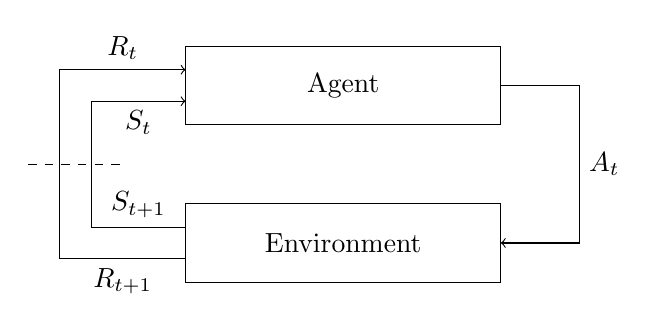
\begin{tikzpicture}
        \draw (0, 2) rectangle node {Agent} (4, 3);
        \draw (0, 0) rectangle node {Environment} (4, 1);

        \draw [->] (4, 2.5) -- (5, 2.5) -- node[right] {$A_t$} (5, 0.5) -- (4, 0.5);

        \draw [->] (0, 0.3) -- node[below] {$R_{t+1}$} (-1.6, 0.3) -- (-1.6, 2.7) --node[above] {$R_t$}  (0, 2.7);
        \draw [->] (0, 0.7) -- node[above] {$S_{t+1}$} (-1.2, 0.7) -- (-1.2, 2.3) -- node[below] {$S_t$} (0, 2.3);

        \draw [dashed] (-2, 1.5) -- (-0.8, 1.5);
    \end{tikzpicture}
    \caption{The agent-environment feedback loop in a Markov Decision Process.}
    \label{fig:mdp_visualization}
\end{figure}

In a \textit{finite Markov Decision Process} \cite{bible}, the sets of states $\mathscr{S}$, actions $\mathscr{A}(s) : \forall s \in \mathscr{S}$, and rewards $\mathscr{R}$ are all finite. With this constraint, we can create a function $p : \mathscr{S} \times \mathscr{R} \times \mathscr{S} \times \mathscr{A} \to \left[0, 1\right]$ to denote probabilities of state transitions occurring. For example, $p\left(s', r \given s, a\right)$ refers to the probability of seeing state $s'$ and receiving reward $r$ after taking action $a$ in state $s$. This implies that transition probabilities are only dependent on the current state and action, but not on historical information.

Usually, an agent is not supposed to focus solely on choosing the action $A_t$ which results in the highest \textit{immediate reward} $R_{t+1}$. Instead, future rewards should also be taken into consideration. Formally, we define the \textit{return} $G_t$ for timestep $t$, which is the sum of all rewards at subsequent timesteps until the final timestep $T$.
\begin{equation*}
    G_t = R_{t+1} + R_{t+2} + R_{t+3} + ... + R_T
\end{equation*}
Accordingly, an agent shall aim to maximize the expected return at each step. The concept of a final timestep only applies to tasks that have a clearly defined beginning and end, making them repetitive in nature. We call a single cycle of these repetitive tasks \textit{episode}.

For tasks that can potentially continue indefinitely, i.e. $T = \infty$, $G_t$ may also become infinite and can, therefore, no longer be subject to maximization. To avoid this issue, we introduce a \textit{discount rate} (or \textit{discount factor}) $\gamma \in [0, 1]$, and define the \textit{discounted return} as follows:
\begin{equation*}
    G_t^{(\gamma)} = R_{t+1} + \gamma R_{t+2} + \gamma^2 R_{t+3} + ...
        = \sum_{k=t+1}^T \gamma^{k-t-1} R_k
\end{equation*}
The parameter $\gamma$ determines to what extend the agent prefers rewards in the near over those in the far future. As an example, an agent with $\gamma = 0$ is only concerned with the immediate reward, whereas the same agent with $\gamma = 0.99$ will optimize for a large time window of rewards. Choosing $\gamma < 1$ ensures that $G_t$ will never become infinite.

In some cases, it is not realistic that the agent receives the full state of the environment. For instance, a robot with a camera cannot possibly measure all physical properties of its surroundings at all times. While a well defined \textit{latent state} may exist, the agent is only provided with an \textit{observation} produced by this state instead. These types of environments are modeled as \textit{Partially Observable Markov Decision Processes}, or \textit{POMDPs} \cite{bible}.
\subsubsection{Policy and Value Functions}
An agent's behavior can be described stochastically. We define the \textit{policy} of an agent to be the probability distributions for taking each available action in the respective states. For a state $s \in \mathscr{S}$, a legal action $a \in \mathscr{A}(s)$, and a policy $\pi$, $\pi\left(a \given s\right)$ is the probability that the agent will perform $a$ in $s$. The learning process consists of adapting $\pi$ over time to maximize the expected return \cite{bible}.

The \textit{value} is another useful measure for a reinforcement learning agent. It describes how good it is for the agent, following a specific policy, to be in a specific state. In other words, the value is the expected return for a policy. We define the \textit{state-value function for policy $\pi$} \cite{bible} as
\begin{equation*}
    v_\pi(s) = \mathbb{E}_\pi\left[G_t | S_t = s\right]
             = \mathbb{E}_\pi\left[\sum_{k=0}^\infty \gamma^k R_{t+k+1} \given S_t = s\right], \forall s \in \mathscr{S}
\end{equation*}
for Markov Decision Processes.

State-value functions do not apply to cases in which the agent tries to diverge from its current policy $\pi$. Because of this, we additionally define the \textit{action-value function for policy $\pi$} \cite{bible}, $q_\pi$, as the expected return when taking any action $a \in \mathscr{A}(s)$ in state $s \in \mathscr{S}$, and subsequently following policy $\pi$:
\begin{equation*}
    q_\pi(s, a) = \mathbb{E}_\pi\left[G_t | S_t = s, A_t = a\right]
             = \mathbb{E}_\pi\left[\sum_{k=0}^\infty \gamma^k R_{t+k+1} \given S_t = s, A_t = a\right], \forall s \in \mathscr{S}
\end{equation*}
\subsubsection{Policy-Based Methods}
We now explain one possible approach to optimize an agent's behavior by directly manipulating its parameterized policy $\pi_\theta$ with regards to the expected returns $\mathbb{E}\left[G_t\right]$. Typically, this is done using gradient descent. The REINFORCE algorithm \cite{reinforce} defines an estimate for $\nabla_\theta \mathbb{E}\left[G_t \given S_t \right]$ as $\nabla_\theta \log \pi_\theta\left(A_t \given S_t\right) G_t$, coining the term \textit{policy gradient}. Intuitively, this may be thought of as increasing or decreasing the probability of actions on a given trajectory based on the return of said trajectory.

Because the return of an entire trajectory needs to be determined before adjusting the policy, REINFORCE may, by itself, only be used in episodic tasks where training occurs at the end of an episode.

The regular is prone to high variance, which can slow down learning. A baseline can be introduced, which is shown to remain unbiased and often improves performance: $\nabla_\theta \log \pi_\theta\left(A_t \given S_t\right) \left(G_t - b(S_t)\right)$.
\subsubsection{Value-Based Methods}
In value-based methods, the agent maintains estimates of the state-value or action-value functions to improve its behavior. The key concept to value-based methods is the recursive definition of value functions, known as the \textit{Bellman equation} \cite{bible}:
\begin{align*}
    v_\pi &= \mathbb{E}_\pi \left[G_t \given S_t = s\right] \\
          &= \mathbb{E}_\pi \left[R_t + G_{t+1} \given S_t = s\right] \\
          &= \sum_a \pi\left(a \given s\right) \sum_{s'} \sum_r p\left(s', r \given s, a\right) \left[r + \gamma \mathbb{E}_\pi\left[G_{t+1} \given S_{t+1} = s'\right]\right] \\
          &= \sum_a \pi\left(a \given s\right) \sum_{s'} \sum_r p\left(s', r \given s, a\right) \left[r + \gamma v_\pi\left(s'\right)\right]
\end{align*}
A similar definition can be created for action-value functions:
\begin{equation*}
    q_\pi\left(s, a\right) = \sum_{s'} \sum_r p\left(s', r \given s, a\right) \left[r + \gamma q_\pi(s', a')\right]
\end{equation*}
The optimal policy, given the correct action-value function, would always perform the action with the highest $q$-value, i.e. expected return. Consequently, the action-values created by this policy are always the highest possible expected returns of any action. This creates a stable condition, known as the \textit{Bellman optimality equation} \cite{bible}, where $q_*$ denotes the action-value function for the optimal policy:
\begin{equation*}
    q_*\left(s, a\right) = \sum_{s'} \sum_r p\left(s', r \given s, a\right) \left[r + \gamma \max_{a'} q_*(s', a')\right]
\end{equation*}

In practice, the transition probabilities $p$ are usually not known. Q-learning \cite{q-learning} approaches this issue by iteratively updating a $q$-value estimates (which we will refer to as $Q$) in a tabular form, known as the Q-table. The iterative formula
\begin{equation*}
    Q\left(S_t, A_t\right) \gets Q\left(S_t, A_t\right) + \beta\left(R_{t+1} + \gamma \max_a Q\left(S_{t+1}, A_t\right) - Q\left(S_t, A_t\right)\right),
\end{equation*}
where $\beta$ is the learning rate hyperparameter, closely resembles the Bellman optimality equation. We are updating the current $Q$-value using the acquired information $R_{t+1}$ as well as a future, \textit{bootstrapped} value estimate: $\max_a Q\left(S_{t+1}, A_t\right)$. This form of learning from future estimates is referred to as \textit{temporal-difference learning} or \textit{TD learning} \cite{td-learning}. The difference between the current estimate and the bootstrapped estimated combined with new experience is called the \textit{TD error}.

Note that Q-learning, similarly to other value-based methods, requires discrete, finite actions, whereas the aforementioned REINFORCE algorithm can handle continuous action spaces. To define a Q-table, the number of possible environment states must also be finite. However, unlike REINFORCE, Q-learning is an \textit{online} algorithm, meaning it can learn from data as soon as it is available (while interacting with the environment), and does not need to wait for the end of an episode. Thus, it can be used for non-terminating tasks. \cite{bible}
\subsubsection{Actor-Critic Methods}
\textit{Actor-critic} methods \cite{bible} try to combine policy- and value-based methods to exploit strengths and mitigate the weaknesses of the two parts. The term is inspired by the way an agent following these methods performs actions in the environment using the policy (actor) component and then judges itself using the value (critic) component.

A possible approach is to use the state-value function estimate $v$ as a baseline for the policy gradient:
\begin{equation*}
    \nabla_\theta \mathbb{E}\left[G_t \given S_t \right] \approx \nabla_\theta \log \pi_\theta\left(A_t \given S_t\right) \left(G_t - v_\pi(S_t)\right)
\end{equation*}
We can replace the actual return $G_t$ with the expected return outputted by the action-value function $q_\pi(s, a) = \mathbb{E}_\pi \left[G_t \given S_t = s, A_t = a\right]$:
\begin{equation*}
    \nabla_\theta \mathbb{E}\left[G_t \given S_t \right] \approx \nabla_\theta \log \pi_\theta\left(A_t \given S_t\right) \left(q(S_t, A_t) - v_\pi(S_t)\right)
\end{equation*}
Note that the term $q(S_t, A_t) - v_\pi(S_t)$ is merely the difference in the value of state $S_t$ when choosing action $A_t$ instead of following policy $\pi_\theta$. Using only a value estimate $V$ of $v_\pi$, this can also be described as $R_{t+1} + \gamma V(S_{t+1}) - V(S_t)$ \cite{a3c}. We call this difference the \textit{advantage} of taking action $A_t$ in state $S_t$. Less formally, the advantage policy gradient can be thought of as increasing the probability of an action whenever the critic is positively surprised by the resulting state, and vice versa.

Updates can be performed online as in Q-learning, and similarly to the default REINFORCE policy gradient, actions must not be discrete. We can see how actor-critics leverage the strengths of both approaches.